\documentclass[11pt,a4paper]{article}

\usepackage[utf8]{inputenc}
\usepackage[T1]{fontenc}
\usepackage[turkish]{babel}
\usepackage{lmodern}
\usepackage[a4paper,margin=2.4cm]{geometry}
\usepackage{setspace}
\onehalfspacing
\usepackage{booktabs}
\usepackage{array}
\usepackage{enumitem}
\setlist[itemize]{itemsep=0.2em,topsep=0.3em}
\setlist[enumerate]{itemsep=0.2em,topsep=0.3em}
\usepackage{graphicx}
\usepackage{subcaption}
\usepackage{amsmath}
\usepackage{tikz}
\usetikzlibrary{shapes.geometric,arrows.meta,positioning}
\usepackage[colorlinks=true,linkcolor=black,urlcolor=blue,citecolor=black]{hyperref}
\usepackage{titlesec}
\titleformat{\section}{\normalfont\large\bfseries}{\thesection}{1em}{}
\titleformat{\subsection}{\normalfont\normalsize\bfseries}{\thesubsection}{1em}{}

\addto\captionsturkish{\renewcommand{\abstractname}{Özet}}
\newcommand{\code}[1]{\texttt{#1}}
\graphicspath{{figures/}{report/figures/}}
\hyphenation{na-vi-gas-yon en-ge-li da-vra-nış klo-nla-ma po-li-ti-ka}

\title{\textbf{MuJoCo Ortamında LNN/CfC Odaklı\\Öğrenmeli Robot Navigasyonu}}
\author{Orkun Koray GÜNGÖR \\ \small{Okul No: 25462877008}}
\date{6 Mayıs 2026}

\begin{document}
\shorthandoff{=}
\maketitle

% =====================================================================
\begin{abstract}
\noindent
Bu çalışmada diferansiyel sürüşlü bir mobil robotun MuJoCo simülasyon
ortamında 32 ışınlı LiDAR gözlemi kullanarak engel içeren haritalarda
hedefe ulaşması incelenmiştir.
Projenin odak noktası, Liquid Neural Network / Closed-form Continuous-time
(LNN/CfC) tabanlı politikayı GRU ve LSTM gibi klasik yinelemeli ağlarla
aynı koşullar altında karşılaştırmaktır.
Proje üç temel adımda yürütülmüştür: (1) MuJoCo tabanlı navigasyon
ortamının ve sensör sözleşmesinin kurulması, (2) GRU ile referans baseline
oluşturulması ve (3) CfC politikasının neden başarısız olduğunun araştırılıp
düzeltilmesi.
Referans yöntem olan GRU, Davranış Klonlama (BC) ve DAgger ile eğitilerek
iki manuel haritada 4/4 başarı elde etmiştir.
CfC politikasında tespit edilen üç mimari ve yapılandırma hatası giderildikten
ve iki DAgger iterasyonu uygulandıktan sonra CfC, altı haritalık test setinde
2 haritada tam başarı, kalan 4 haritada çarpışmasız navigasyon sağlamıştır.

\vspace{0.5em}
\noindent\textbf{Anahtar sözcükler:}
mobil robot navigasyonu, MuJoCo, LiDAR, LNN, CfC, GRU,
davranış klonlama, DAgger.
\end{abstract}

% =====================================================================
\section{Konu ve Planlama}

\subsection{Odak Konu}

Bu projede araştırılan soru şudur: \emph{Sürekli zamanlı yinelemeli ağ
mimarileri (LNN/CfC), kısa menzilli LiDAR gözlemiyle engel içeren
bir ortamda navigasyon öğrenmede GRU'ya kıyasla nasıl bir başarım gösterir?}

Konu motivasyonu üç gözleme dayanmaktadır:
\begin{itemize}
  \item CfC, sabit zaman adımına bağımlı olmayan sürekli zamanlı ODE
  dinamiğiyle çalışır; bu özellik değişken kontrol frekanslarında avantaj
  sağlayabilir.
  \item Navigasyon görevi kısmi gözlem altında ardışık karar verme gerektirir;
  yinelemeli ağların gizli durumu bu geçmiş bilgiyi taşır.
  \item CfC uygulamalarında rapor edilen başarımı doğrulamak için robotik
  navigasyon gibi gerçek bir kontrol görevinde bağımsız değerlendirme
  yapılmamıştır.
\end{itemize}

\subsection{Proje Planı}

Tablo~\ref{tab:plan} tüm proje adımlarını ve güncel durumlarını özetlemektedir.

\begin{table}[h]
\centering
\caption{Proje planı ve adım durumları}
\label{tab:plan}
\begin{tabular}{clp{6.8cm}l}
\toprule
\textbf{\#} & \textbf{Adım} & \textbf{İçerik} & \textbf{Durum} \\
\midrule
1 & Ortam & MuJoCo diferansiyel sürüş ortamı, harita editörü,
           LiDAR sensör modeli & Tamamlandı \\
2 & Baseline & GRU + BC/DAgger ile referans politika,
              iki haritada saf politika değerlendirmesi & Tamamlandı \\
3 & CfC analizi & CfC başarısızlığının kök neden analizi
                 ve mimari düzeltme & Tamamlandı \\
4 & Karşılaştırma & 6 haritalık test setinde GRU, CfC, LSTM, MLP
                   adil karşılaştırması & Tamamlandı \\
5 & OOD testleri & Sensör gürültüsü ve görülmemiş (holdout)
                  haritalarda dayanıklılık değerlendirmesi & Sonraki adım \\
\bottomrule
\end{tabular}
\end{table}

% =====================================================================
\section{Ortam ve Sensör Modeli}

Simülasyon ortamı \code{mujoco} Python API'siyle kurulmuştur.
Robot; zemin üzerindeki silindir, kutu ve çizgi/duvar engel kombinasyonlarını
içeren haritalarda hareket eder.
Tüm eğitim ve değerlendirme headless modda çalışmış, sonuçlar üstten görünüm
PNG/GIF çıktılarıyla görselleştirilmiştir.

\begin{center}
\begin{tabular}{lc}
\toprule
\textbf{Gözlem bileşeni} & \textbf{Boyut} \\
\midrule
Normalize hedef mesafesi & 1 \\
Normalize hedef açısı & 1 \\
Doğrusal ve açısal hız & 2 \\
Önceki aksiyon & 2 \\
32 LiDAR/range ışını & 32 \\
\midrule
\textbf{Toplam} & \textbf{38} \\
\bottomrule
\end{tabular}
\end{center}

Aksiyon: \code{[linear, angular]} $\in [-1, 1]^2$. \\
Fizik adımı: \code{physics\_dt} $= 0.02\,\text{s}$, \code{frame\_skip} $= 4$,
kontrol döngüsü $\Delta t = 0.08\,\text{s}$.

% =====================================================================
\section{Temel Yöntem: GRU + BC/DAgger}

\subsection{Eğitim Hattı}

Şekil~\ref{fig:pipeline} eğitim hattını özetlemektedir.

\begin{figure}[h]
\centering
\begin{tikzpicture}[
  box/.style={rectangle,draw,rounded corners=3pt,minimum width=2.8cm,
              minimum height=0.9cm,align=center,font=\small,fill=blue!7},
  teach/.style={rectangle,draw,rounded corners=3pt,minimum width=2.8cm,
                minimum height=0.9cm,align=center,font=\small,fill=orange!15},
  arr/.style={-{Stealth[length=2.5mm]},thick},
  node distance=0.55cm and 1.1cm
]
\node[box] (map)   {MuJoCo\\haritası};
\node[teach,right=of map] (astar) {A* öğretmen\\planlayıcı};
\node[box,right=of astar] (demo)  {Gözlem--\\aksiyon çifti};
\node[box,right=of demo]  (bc)    {BC eğitimi\\(MSE kayıp)};
\node[box,below=0.9cm of bc] (dag)   {DAgger\\iterasyonu};
\node[box,left=of dag]   (roll)  {Politika\\rollout'u};
\node[teach,left=of roll]  (label) {Öğretmen\\yeniden etiket};
\draw[arr] (map) -- (astar);
\draw[arr] (astar) -- (demo);
\draw[arr] (demo) -- (bc);
\draw[arr] (bc) -- (dag);
\draw[arr] (dag) -- (roll);
\draw[arr] (roll) -- (label);
\draw[arr] (label.north) -- ++(0,0.4) -| (demo.south);
\node[font=\footnotesize,gray] at (4.5,-1.9) {A* yalnızca eğitimde; eval'de kapalı};
\end{tikzpicture}
\caption{Eğitim hattı: BC ve DAgger aşamaları}
\label{fig:pipeline}
\end{figure}

\textbf{Davranış Klonlama (BC):}
A* tabanlı öğretmen her haritada referans yollar üretir.
Model, bu yollar boyunca toplanan $\langle$gözlem, aksiyon$\rangle$ çiftlerini
taklit etmek üzere eğitilir.
Kayıp fonksiyonu ağırlıklı MSE'dir; engel yakınındaki adımlara ve yolun
başına daha yüksek ağırlık verilir.

\textbf{DAgger:}
Mevcut politika kendi kararlarıyla ortamı dolaşır; öğretmen bu durumlara da
yeni etiket üretir ve politika yeni durumlarla iyileştirilir.
Bu yineleme, BC'nin dağılım kayması sorununu azaltır.

\subsection{GRU Mimarisi}

Gizli durum boyutu 128, giriş kodlayıcısı \code{Linear(38,128)+Tanh},
ardından 128 birimlik GRU hücresi, çıkışta \code{Linear(128,2)} aksiyon
başlığı ve \code{Linear(128,1)} değer başlığı bulunmaktadır.
Eğitimde politika Adam optimize edici ($\text{lr}=5\!\times\!10^{-4}$)
ve gradyen kırpması (norm $\leq 1.0$) ile güncellenmiştir.

% =====================================================================
\section{Sonuçlar: GRU Baseline}

\subsection{Vize Değerlendirmesi — 2 Manuel Harita}

Tablo~\ref{tab:vize} vize aşamasında elde edilen sonuçları göstermektedir.
Değerlendirme A* kapalı, saf politika modundadır.

\begin{table}[h]
\centering
\caption{GRU + BC/DAgger baseline — 2 harita, 4 bölüm, max-steps = 900}
\label{tab:vize}
\begin{tabular}{lcccc}
\toprule
\textbf{Harita} & \textbf{Başarı} & \textbf{Çarpışma} & \textbf{Ort.\ Adım} & \textbf{Son mesafe (m)} \\
\midrule
\code{custom\_map\_01} & 1.00 & 0.00 & 459 & 0.20 \\
\code{custom\_map\_02} & 1.00 & 0.00 & 521 & 0.19 \\
\bottomrule
\end{tabular}
\end{table}

Her iki haritada da 4 bölümün tamamı başarıyla tamamlanmıştır.

\subsection{Rollout Görselleri}

Şekil~\ref{fig:rollouts} her iki haritadaki başarılı rollout yollarını
LiDAR ışınlarıyla birlikte göstermektedir.
Engeller turuncu/kırmızı kutular ve silindirlerle, robot yolu mavi çizgiyle,
hedef yeşil daire ile belirtilmiştir.

\begin{figure}[h]
\centering
\begin{subfigure}[b]{0.47\linewidth}
  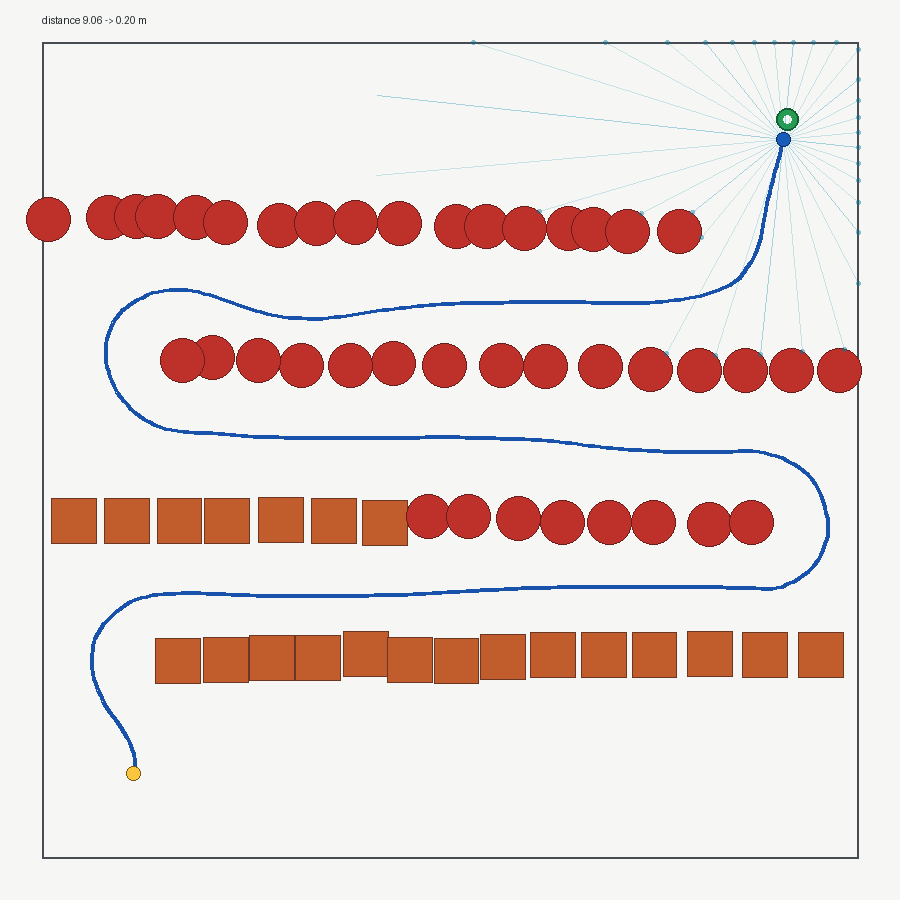
\includegraphics[width=\linewidth]{custom_map_01_lidar.png}
  \caption{\code{custom\_map\_01} — dar koridor, 459 adım}
  \label{fig:map01}
\end{subfigure}
\hfill
\begin{subfigure}[b]{0.47\linewidth}
  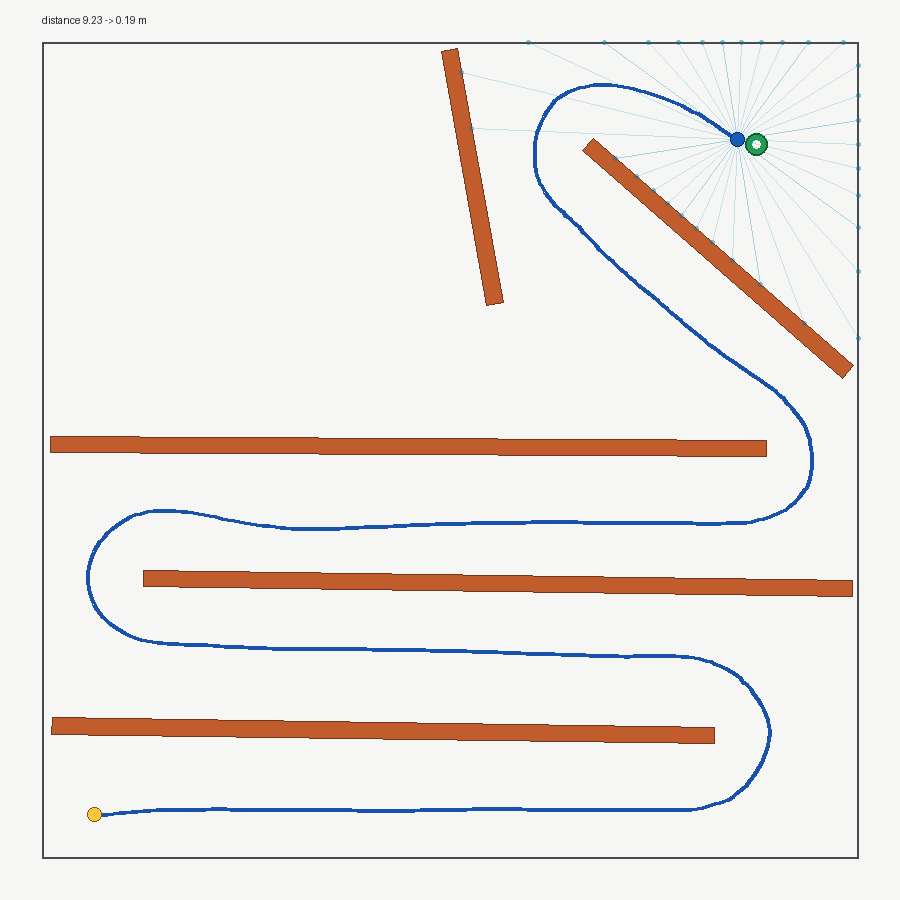
\includegraphics[width=\linewidth]{custom_map_02_lidar.png}
  \caption{\code{custom\_map\_02} — L şekilli geçit, 521 adım}
  \label{fig:map02}
\end{subfigure}
\caption{GRU politikasının iki manuel haritadaki başarılı rollout yolları}
\label{fig:rollouts}
\end{figure}

% =====================================================================
\section{CfC Politikası: Başarısızlık Analizi ve Düzeltme}

\subsection{Başarısızlık Gözlemi}

CfC politikası aynı eğitim hattına eklendiğinde sekiz haritalık test setinde
tüm bölümlerde çarpışma ve sıfır başarı üretmiştir.
Eğitim kaybı ise $\approx 0.001$ gibi düşük değerlere ulaşmıştı.
Düşük kayıp + sıfır başarı: uzman durum dağılımında iyi taklit, ancak
kendi hata durumlarında hızla sapma (dağılım kayması).

\subsection{Tespit Edilen Kök Nedenler}

\begin{enumerate}
\item \textbf{Giriş kodlayıcısı eksikliği (en kritik).}
GRU mimarisinde ham gözlem önce \code{Linear(38,128)+Tanh} ile ortak
gizli alana yansıtılır.
CfC ise 38 boyutlu ham gözlemi (LiDAR $\in [0,1]$, hız $\approx\pm5$,
açı $\in [-\pi,\pi]$) doğrudan ODE hücresine veriyordu;
bu ölçek farkı öğrenmeyi zorlaştırmaktaydı.

\item \textbf{Asimetrik eğitim bütçesi.}
GRU: 500 dönem, harita başına 4 bölüm (24 demo).
CfC: 220 dönem, harita başına 2 bölüm (12 demo).
CfC, GRU'nun yarısı kadar veriyle eğitiliyordu.

\item \textbf{ODE zaman adımı hatası.}
\code{ncps.torch.CfC} varsayılanı $\Delta t = 1.0\,\text{s}$'dir;
gerçek kontrol adımı ise $0.08\,\text{s}$.
ODE çözücüsü her adımda $12.5\times$ fazla zaman ilerletiyordu.
\end{enumerate}

\subsection{Uygulanan Düzeltmeler}

\begin{enumerate}
\item \code{CfCActorCritic}'e GRU ile özdeş giriş kodlayıcısı eklendi:
      \code{self.input = nn.Sequential(Linear(38,128), Tanh())}.
\item CfC eğitim yapılandırması GRU ile eşitleştirildi:
      500 dönem, harita başına 4 bölüm, yığın büyüklüğü 2.
\item Tüm CfC ileri geçişlerine $\Delta t = 0.08\,\text{s}$ iletildi.
      \code{ncps} kütüphanesinin iç döngüsünde skalar beklentisini
      karşılamak üzere zaman tensörü $(1, T)$ boyutunda oluşturuldu.
\end{enumerate}

% =====================================================================
\section{Final Karşılaştırması}

\subsection{Eğitim Kaybı}

500 dönem sonunda:

\begin{center}
\begin{tabular}{lcc}
\toprule
\textbf{Model} & \textbf{İlk kayıp} & \textbf{Son kayıp} \\
\midrule
GRU (BC)               & 0.120 & $1.26 \times 10^{-4}$ \\
CfC düzeltilmiş (BC)   & 0.122 & $7.44 \times 10^{-5}$ \\
\bottomrule
\end{tabular}
\end{center}

Düzeltilmiş CfC, eğitim kaybı açısından GRU'yu geride bırakmıştır.

\subsection{Saf Politika Değerlendirmesi — 6 Harita}

Tablo~\ref{tab:final} üç modeli aynı koşullarda karşılaştırmaktadır
(4 bölüm, max-steps = 900, A* kapalı).

\begin{table}[h]
\centering
\caption{6 haritada saf politika değerlendirmesi}
\label{tab:final}
\begin{tabular}{lcccccc}
\toprule
 & \multicolumn{2}{c}{\textbf{GRU BC}} &
   \multicolumn{2}{c}{\textbf{CfC kırık}} &
   \multicolumn{2}{c}{\textbf{CfC düzeltilmiş}} \\
\cmidrule(lr){2-3}\cmidrule(lr){4-5}\cmidrule(lr){6-7}
\textbf{Harita} & Başarı & Adım & Başarı & Adım & Başarı & Adım \\
\midrule
\code{map\_01} & 0.00 &  93 & 0.00 &  55 & \textbf{1.00} & 445 \\
\code{map\_02} & 0.00 & 312 & 0.00 &  19 & 0.00 & 900$^\dagger$ \\
\code{map\_04} & 0.00 & 126 & 0.00 & 161 & 0.00 & 900$^\dagger$ \\
\code{map\_05} & 0.00 & 648 & 0.00 & 128 & 0.00 & 900$^\dagger$ \\
\code{map\_06} & 0.00 & 103 & 0.00 & 103 & 0.00 & 900$^\dagger$ \\
\code{map\_07} & 0.00 & 242 & 0.00 & 180 & \textbf{1.00} & 231 \\
\midrule
\textbf{Başarı toplamı} & \multicolumn{2}{c}{0/6} &
                          \multicolumn{2}{c}{0/6} &
                          \multicolumn{2}{c}{\textbf{2/6}} \\
\bottomrule
\multicolumn{7}{l}{$\dagger$ Timeout: çarpışmasız 900 adım, hedefe ulaşılamadı.}
\end{tabular}
\end{table}

Düzeltme öncesi CfC tüm haritalarda çarpışma üretirken,
düzeltme sonrası 2 haritada tam başarı ve 4 haritada çarpışmasız navigasyon
elde edilmiştir.
Timeout gözlemleri modelin engelleri tanıdığını ancak uzun vadeli
hedef takibini henüz tam öğrenemediğini göstermektedir.

% =====================================================================
\section{Sonuç}

Bu çalışmada MuJoCo tabanlı bir navigasyon ortamı kurulmuş, GRU ile başarılı
bir referans yöntem oluşturulmuş ve CfC politikasının neden sıfır başarı
ürettiği sistematik biçimde araştırılmıştır.

Tespit edilen üç sorun --- giriş kodlayıcısı eksikliği, asimetrik eğitim
bütçesi ve yanlış ODE zaman adımı --- giderildikten sonra CfC, 6 haritanın
2'sinde tam başarı ve tüm haritalarda çarpışmasız hareket elde etmiştir.
Bu sonuçlar, CfC'nin eşit mimari koşullar ve doğru ODE entegrasyonu altında
GRU ile rekabetçi hale gelebildiğini göstermektedir.

Sonraki adımda holdout haritaları ve sensör gürültüsü altında dayanıklılık
değerlendirmesi planlanmaktadır.

\vspace{0.5em}
\noindent\textbf{Kod:}
\url{https://github.com/heimdilon/mujoco_lnn_navigation}

\end{document}
